\documentclass[fr]{../../../eplnotes}

\usepackage{../../../eplunits}
\usepackage{../../../eplmeca}


\hypertitle{Mécanique}{2}{EPL}{1202}
{Louis Devillez}
{Paul Fisette}[
\paragraph{Remarque}
Ce document a pour objectif de rassembler les démonstrations importantes du cours en vue de l'examen. Il suppose une compréhension préalable de la matière et ne fait office ni de synthèse, ni de syllabus.
]

%\begin{document}


\section{Changement de base: composante d'un vecteur}

	\begin{align*}
		\bf{u} &= \{\ui\}^t  u_i\\
		\{\ux\} = A \{\ui\}	&\Rightarrow \{\ui\}^t = \{\ux\}^t A \\
		\bf{u} &= \{\ux\}^t A  u_i \\
		u_x &= A u_i
 	\end{align*}	
 	
 	
\section{Changement de base: matrice tilde}
	\begin{align*}
		\bf{u} \times \bf{v} &= \{\ui\}^t \tilde{u_i}v_i\\
		&= \{\ux\}^t \tilde{(Au_i)} Av_i\\
		\{\ui\}^t \tilde{u_i}v_i&= \{\ux\}^t \tilde{(Au_i)} Av_i\\
		\{\ux\}^t A \tilde{u_i}v_i&= \{\ux\}^t \tilde{(Au_i)} Av_i\\
		A\tilde{u_i}&=\tilde{(Au_i)} A\\
		\tilde{(Au_i)}&=A\tilde{u_i}A^t
	\end{align*} 

\section{Dérivée d'un vecteur exprimé dans une base mobile}
	\begin{align*}
		\bf{u} &= \{\ui\}^t  A^t u_x\\
		\dot{\bf{u}} &= \{\ui\}^t (\dot{A^t} u_x + A^t\dot{u}_x)\\
		&= \{\ux\}^t (A\dot{A^t} u_x + \underbrace{AA^t}_{=E}\dot{u}_x)\\
		&= \{\ux\}^t (A\dot{A^t} u_x + \dot{u}_x)
	\end{align*}
	Nous posons que $A\dot{A^t} = \tilde{\omega}$ car cette matrice est anti-symétrique
	\begin{align*}
		A A^t &= E\\
		\dot{A} A^t + A \dot{A^t} &= 0\\
		\dot{A} A^t &=- A \dot{A^t}\\
		\dot{A} A^t &= -(\dot{A} A^t)^t
	\end{align*}
	et peut s'écrire sous la forme
	\begin{eqnarray*}
	A A^t = \begin{pmatrix}0 & -\omega_3 & \omega_2\\ \omega_3 & 0 & -\omega_1\\ -\omega_2 & \omega_1 & 0\end{pmatrix}
	\end{eqnarray*}
	nous obtenons alors
		\begin{align*}
		\dot{\bf{u}} &= \{\ux\}^t (\dot{u}_x + \tilde{\omega}u_x)\\
		\dot{\bf{u}} &= \mathring{\bf{u}} + \bf{\omega} \times \bf{u}
		\end{align*}


\section{Dérivée seconde d'un vecteur exprimé dans une base mobile}
Nous allons réutiliser l'opérateur dérivée trouvé dans le section précédente
	\begin{align*}
		\ddot{\bf{u}} &= \{\ux\}^t (\ddot{{u}_x} + \dot{\tilde{\omega}}u_x +  \tilde{\omega}\dot{u_x}) +  \{\ux\}^t \tilde{\omega} (\dot{u}_x + \tilde{\omega}u_x)\\
		&= \{\ux\}^t (\ddot{{u}_x} + \dot{\tilde{\omega}}u_x + 2 \tilde{\omega}\dot{u_x} +\tilde{\omega}\tilde{\omega} u_x)\\
		&=\overset{\circ\circ}{\bf{u}} + 2 \bf{\omega} \times \mathring{\bf{u}} + \mathring{\bf{\omega}} \times \bf{u} + \bf{\omega} \times(\bf{\omega} \times \bf{u})
	\end{align*}
\section{Composition des vecteurs vitesses angulaires}
	 Soit 
	\begin{align*}
		\{\ux\} &= A_1 \{\ui\} \\
		\{\uy\} &= A_2 \{\ux\}
	\end{align*}
	Nous pouvons en déduire que
	$$
		\{\uy\} = A_2 A_1 \{\ui\}\\
	$$
	Nous pouvons dès maintenant rechercher nos vecteurs $\omega$
	\begin{align*}
		\tilde{\omega}^{XI} &= A_1\dot{A_1}^t\\
		\tilde{\omega}^{YX} &= A_2\dot{A_2}^t\\
		\tilde{\omega}^{YI} &= A_2A_1(\dot{A_2}A_1 + A_2\dot{A_1})^t\\
		&= A_2A_1(A_1^t\dot{A^t_2} + \dot{A^t_1}A_2^t)\\
		&= A_2\underbrace{A_1A_1^t}_{= E}\dot{A^t_2} + A_2A_1\dot{A^t_1}A_2^t\\
		&= \tilde{\omega}^{YX} + A_2\tilde{\omega}^{XI}A_2^t\\
		&= \tilde{\omega}^{YX} + \tilde{(A_2\omega^{XI})}\\
	\end{align*}
	Nous pouvons retirer le $\sim$  n'étant que représentation particulière d'un vecteur
	\begin{align*}
		\bf{\omega^{YI}} = \{\uy\}^t \omega^{YI} &= \{\uy\}^t A_2 \omega^{XI} + \{\ui\}^t \omega^{YX}\\
		&= \{\ux\}^t \omega^{XI} + \{\ui\}^t \omega^{YX}\\
		\bf{\omega^{YI}} &= \bf{\omega^{XI}} +\bf{\omega^{YX}}
	\end{align*}
	
\section{Vecteur position du centre de masse}

\begin{center}
	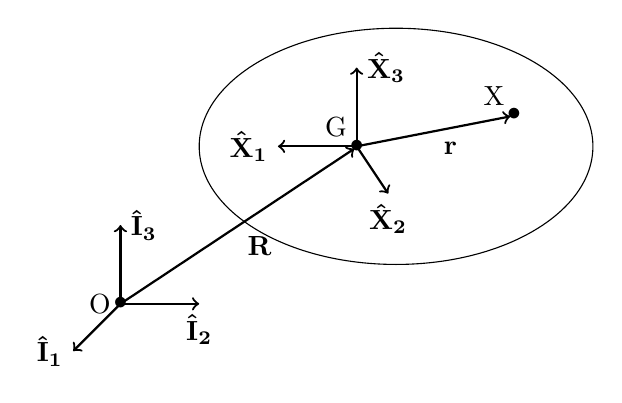
\begin{tikzpicture}
		 \draw (0,0) [->,thick] -- (0,1) node[anchor=west]{$\bf{\hat{I}_3}$};
		 \draw (0,0) [->,thick] -- (1,0) node[anchor=north]{$\bf{\hat{I}_2}$};
		 \draw (0,0) [->,thick] -- (-0.6,-0.6) node[anchor=east]{$\bf{\hat{I}_1}$};
		 \draw (0,0) node[]{$\bullet$} node[anchor =east]{O};
		 
		 \draw (3.5,2) circle (2.5 and 1.5);
		 \draw (0,0) [->,thick] -- (2.97,1.97) node[midway, anchor= north west]{$\bf{R}$};
		 \draw (3,2) node[]{$\bullet$} node[anchor = south east]{G};
		 
		 \draw (3,2) [->,thick] -- (3,3) node[anchor=west]{$\bf{\hat{X}_3}$};
		 \draw (3,2) [->,thick] -- (3.4,1.4) node[anchor=north]{$\bf{\hat{X}_2}$};
		 \draw (3,2) [->,thick] -- (2,2) node[anchor=east]{$\bf{\hat{X}_1}$};
		 
		 \draw (3,2) [->,thick] -- (4.95,2.38) node[midway,anchor=north west]{$\bf{r}$};
		 \draw (5,2.4) node[]{$\bullet$} node[anchor = south east]{X};
	\end{tikzpicture}
\end{center}

	$$
	\bf{OX} = \bf{x} = \bf{R(t)} + \bf{r(t)}
	$$
	R indiquant le centre de masse
	\begin{align*}
		\bf{R(t)} &= \frac{1}{m} \int_C \bf{x} \dif m\\
		&= \frac{1}{m} \int_C \bf{R} \dif m + \frac{1}{m} \int_C \bf{r} \dif m\\
		&= \frac{1}{m} \bf{R} \int_C  \dif m + \frac{1}{m} \int_C \bf{r} \dif m\\
		0 &= \frac{1}{m} \int_C \bf{r} \dif m\\
	\end{align*}
	On peut en conclure que le centre de masse est la moyenne pondérée des points matériels composant un corps.

	
\section{Vecteur quantité de mouvement}
	\begin{align*}
		\bf{N}^i & = m^i \dot{\bf{x^i}}\\
		&= m * (\frac{1}{m} \int_C \dot{\bf{R}} \dif m + \frac{1}{m} \int_C \bf{\omega}\times \bf{r} \dif m)\\
		&= m \dot{\bf{R}} + \bf{\omega} \times \underbrace{\int_C \bf{r} \dif m}_{=0}\\
		&=m \dot{\bf{R}}
	\end{align*}
	
	
	
\section{Vecteur moment de la quantité de mouvement par rapport un point P}

	\begin{align*}
		\bf{\am^p}& = \int_C \bf{PX} \times \dot{\bf{PX}} \dif m\\
		&=\{\ux\}^t \int_C \tilde{p} * \tilde{\omega} p\dif m =\{\ux\}^t - \int_C \tilde{p}\tilde{p} \omega \dif m\\
		&= \{\ux\}^t I^p \omega
	\end{align*}
	
	
\section{Vecteur moment de la quantité de mouvement par rapport au centre de masse}
	\begin{align*}
		\bf{\am^G}& = \int_C \bf{GX} \times \dot{\bf{GX}} \dif m\\
		&=\{\ux\}^t \int_C \tilde{r} * \tilde{\omega} r\dif m =\{\ux\}^t - \int_C \tilde{r}\tilde{r} \omega \dif m\\
		&= \{\ux\}^t I^G \omega
	\end{align*}
	
	
\section{Vecteur moment de la quantité de mouvement par rapport à O}
	\begin{align*}
		\bf{x} &= \bf{R} + \bf{r}\\
		\bf{\am^0} & = \int_C \bf{x} \times \dot{\bf{x}} \dif m\\
		&= \int_C (\bf{R} + \bf{r}) \times (\mathring{\bf{R}} +\tilde{\omega} R+\mathring{\bf{r}} + \tilde{\omega}r) \dif m\\
		&= - \int_C \tilde{R} \tilde{R} \omega \dif m - \int_C \tilde{r} \tilde{r} \omega \dif m \\
		&= \bf{\am^G} - m \tilde{R}\tilde{R}
	\end{align*}
	Le produit vectoriel nous donne bien que deux termes car:
	\begin{itemize}
		\item Soit les vecteurs ont même direction ce qui donne bien 0 ;
		\item Soit r est constant et donc $\mathring{r}$ donne 0 ;
		\item Soit $\int_C r \dif m$ et $\int_C \tilde{r} \dif m$ nous donne 0.
	\end{itemize}
	
\section{Energie cinétique}
	\begin{align*}
		\bf{T}(t) &= \frac{1}{2} \int_C \dot{\bf{x(t)}} \dot{\bf{x(t)}} \dif m \\
		&=\frac{1}{2} m \dot{\bf{R(t)}} \dot{\bf{R(t)}} + \frac{1}{2} \int_C \dot{\bf{r(t)}} \dot{\bf{r(t)}} \dif m\\
		 &= \frac{1}{2} m \dot{\bf{R(t)}} \dot{\bf{R(t)}} + \frac{1}{2} \int_C (\tilde{r}\omega) (\tilde{r} \omega) \dif m\\
		 &= \frac{1}{2} m \dot{\bf{R(t)}} \dot{\bf{R(t)}} + \frac{1}{2} \int_C -(\tilde{r}\omega)^t (\tilde{r} \omega) \dif m\\
		 &= \frac{1}{2} m \dot{\bf{R(t)}} \dot{\bf{R(t)}} + \frac{1}{2} \int_C -\omega^t\tilde{r} \tilde{r} \omega \dif m\\
		 &= \frac{1}{2} m \dot{\bf{R(t)}} \dot{\bf{R(t)}} + \frac{1}{2} \omega^t \int_C -\tilde{r}\tilde{r} \dif m *\omega\\
		 &= \frac{1}{2} m \dot{\bf{R(t)}} \dot{\bf{R(t)}} + \frac{1}{2} \omega^t I^G \omega\\
	\end{align*}
	
	
\section{Théorème de Steiner}

\begin{center}
	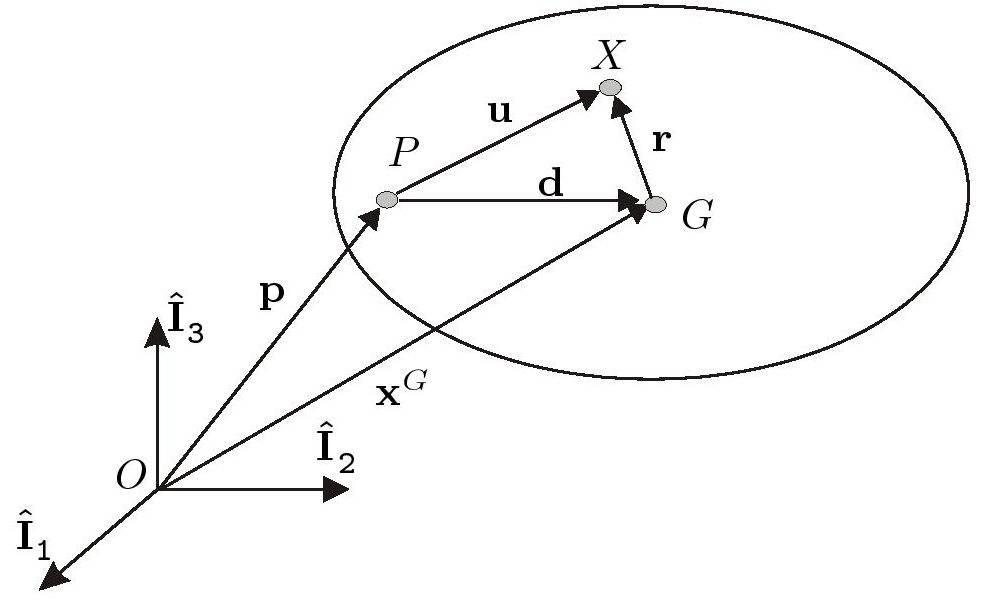
\includegraphics[width=.5\textwidth]{notation.png}
\end{center}

	\begin{align*}
		\bf{PX} &= \bf{PG} + \bf{GX}\\
		\ine^P & = \int_C \bf{PX} \times \dot{\bf{PX}} \dif m\\
		&= \int_C (\bf{d} + \bf{r}) \times (\mathring{\bf{d}} +\tilde{\omega} d+\mathring{\bf{r}} + \tilde{\omega}r) \dif m\\
		&= - \int_C \tilde{d} \tilde{d} \omega \dif m - \int_C \tilde{r} \tilde{r} \omega \dif m \\
		&= \ine^G - m \tilde{d}\tilde{d}
	\end{align*}
	Le produit vectoriel nous donne bien que deux termes car:
	\begin{itemize}
		\item Soit les vecteurs ont même direction ce qui donne bien 0 ;
		\item Soit r est constant et donc $\mathring{r}$ donne 0 ;
		\item Soit $\int_C r \dif m$ et $\int_C \tilde{r} \dif m$ nous donne 0.
	\end{itemize}
	
	
\section{Changement de base de la matrice d'inertie}
	\begin{align*}
		\{\uy\} &= B \{\ui\}\\
		X_y &= B X_x\\
		I_y &= - \int_C \tilde{X_y}\tilde{X_y} \dif m \\
		&= - \int_C \tilde{(B X_x)}\tilde{(BX_x)} \dif m \\
		&= - \int_C B \tilde{X_x} B^t B \tilde{X_x} B^t \dif m \\
		&= BI_x B^t \\
	\end{align*}
	
	
\section{Couple pur}
%TODO schema
Soit $F_1$ et $F_2$ deux forces de même intensité mais opposées et Q un point quelconque du corps.
	\begin{align*}
		L^Q &= \bf{QA} \times F_1 + \bf{QA'} \times F_2\\
		&= \bf{QA} \times F_1 - \bf{QA'} \times F_1\\
		& = (\bf{QA} - \bf{QA'}) \times F_1\\
		& = \bf{AA'} \times F_1
	\end{align*}
	$L^Q$ ne dépend pas de Q, il est donc appelé couple pur.
	
	
\section{Variation potentielle de puissance d'une force}
	\begin{align*}
		\dot{\bf{x}} & = \dot{\bf{R}} + \omega \times \bf{r}\\
		\bf{F} \cdot \Delta\dot{\bf{R}} &= \bf{F} \cdot \Delta\dot{\bf{x}} - \bf{F} \cdot (\Delta\omega \times \bf{r})\\
		&= \bf{F} \cdot \Delta\dot{\bf{x}} - \Delta\omega \cdot (\bf{r}\times \bf{F})\\
		&= \bf{F} \cdot \Delta\dot{\bf{x}} - \bf{L^G} \cdot \Delta \omega\\
		\bf{F} \cdot \Delta\dot{\bf{x}} &= \bf{F} \cdot \Delta\dot{\bf{R}}  + \bf{L^G} \cdot \Delta \omega
	\end{align*}
\section{Forces de contrainte Q'}
Je sais que :
	\begin{align}
	J(q) \Delta \dot{q} &= 0\label{eq1}\\
	Q' \delta \dot{q} &= 0\label{eq2}
	\end{align}
	
De \ref{eq1}, on peut dire que $\Delta \dot{q}$ est le complément orthogonal de $J(q)$.

De \ref{eq2}, on peut dire que $Q'$ est orthogonal au complément orthogonal de $J(q)$.

$Q'$ appartient donc à l'espace des lignes de J $\Leftrightarrow Q'$ est combinaison linéaire des lignes de J.

\begin{align*}
	Q' &= \lambda_1 ligne_1(J) + \lambda_2 ligne_2(J) + ... + \lambda_n ligne_n(J)\\
	Q' &= J^t \lambda
\end{align*}


\end{document}
